\documentclass{anstrans}

%%%% packages and definitions (optional)
\usepackage{color} % allows inclusion of graphics
\usepackage{graphicx} % allows inclusion of graphics
\usepackage{booktabs} % nice rules (thick lines) for tables
\usepackage{microtype} % improves typography for PDF
\usepackage{subcaption}
\usepackage{tikz}

\newcommand{\SN}{S$_N$}
\renewcommand{\vec}[1]{\bm{#1}} %vector is bold italic
\newcommand{\vd}{\bm{\cdot}} % slightly bold vector dot
\newcommand{\ud}{\mathop{}\!\mathrm{d}} % upright derivative symbol
%  new definitions
\newcommand{\bs}[1]{\mathbf{#1}}
\renewcommand{\div}{\bs{\nabla}\! \cdot \!}
\newcommand{\grad}{\bs{\nabla}}
% extra space
\newcommand{\qq}{\quad\quad}
% common reference commands
\newcommand{\eqt}[1]{Eq.~(\ref{#1})}                     % equation
\newcommand{\fig}[1]{Fig.~\ref{#1}}                      % figure
\newcommand{\tbl}[1]{Table~\ref{#1}}                     % table
\newcommand{\sct}[1]{Section~\ref{#1}}                   % section
\newcommand{\app}[1]{Appendix~\ref{#1}}                   % appendix

\newcommand{\keff}{k_\textit{eff}}

\newcommand{\be}{\begin{equation}}
\newcommand{\ee}{\end{equation}}
\newcommand{\vn}{\vec{n}}
\newcommand{\vel}{\vec{\mathrm{v}}}
\newcommand{\adj}{\Phi^\dagger_0}
\newcommand{\tcr}[1]{\textcolor{red}{#1}}
\newcommand{\norm}[1]{\left\lVert#1\right\rVert_{L^2}}

%%%% changes from the original 'anstrans' class
\usepackage{fancyhdr} % allows headers and footers

\renewcommand\headrule{} % remove underline in the header
\setcounter{secnumdepth}{1}
\renewcommand{\thesection}{\Roman{section}.}
\renewcommand{\thesubsection}{\arabic{subsection}.}
\renewcommand{\thesubsubsection}{\Alph{subsubsection}.}
\makeatletter
\renewcommand*{\@seccntformat}[1]{\csname the#1\endcsname\hspace{1mm}}
\makeatother


%%%% Header
\pagestyle{fancy}
\fancyhf{}
\fancyhead[L]{\fontsize{9}{9} \itshape
M\&C 2017 - International Conference on Mathematics \& Computational Methods Applied to Nuclear Science \& Engineering,
\\ Jeju, Korea, April 16-20, 2017, on USB (2017)
}


%%%% Maketitle
\title{Multiphysics Core Dynamics Simulation Using the Improved Quasi-Static Method}
\author{Zachary M.~Prince, Jean C.~Ragusa}

\institute{Department of Nuclear Engineering, Texas A\&M University, College Station, TX}

\email{zachmprince@tamu.edu \and jean.ragusa@tamu.edu}

% tikz stuff
\usetikzlibrary{shapes,arrows,positioning}
\pgfdeclarelayer{background}
\pgfdeclarelayer{foreground}
\pgfsetlayers{background,main,foreground}
\tikzstyle{greenblock}=[rectangle, rounded corners, draw, align=center, top color=white, bottom color=green!20, ultra thick, minimum width=60mm, minimum height=15mm,]
\tikzstyle{blueblock}=[rectangle, rounded corners, draw, align=center, top color=white, bottom color=blue!20, ultra thick, minimum width=60mm, minimum height=15mm]
\tikzstyle{reddiamond}=[diamond, draw, align=center, top color=white, bottom color=red!20, ultra thick, minimum width=60mm, aspect=2]

%%%% Abstract
\begin{document}
\vspace*{-42pt}
\begin{strip}
\centering{\parbox{153mm}{{\bf Abstract} \itshape - 
This template provides the standard format and styles of the full papers to be submitted to M\&C 2017. It is basically the same as the extended summary template except that the abstract is given and the section numbers are specified.
}\par}
\vspace*{14pt}
\end{strip}


%%%%%%%%%%%%%%%%%%%%%%%%%%%%%%%%%%%%%%%%%%%%%%%%%%%%%%%%%%%%%%%%%%%%%%%%%%%%%%%%
\section{Introduction}
%%%%%%%%%%%%%%%%%%%%%%%%%%%%%%%%%%%%%%%%%%%%%%%%%%%%%%%%%%%%%%%%%%%%%%%%%%%%%%%%

The purpose of this paper is to introduce several techniques in dealing with multi-physics feedback for transient neutron diffusion calculations.  In dynamic simulations, the neutron temporal distribution in a nuclear core can be strongly influenced by non-neutronics variables, e.g., temperature.The improved quasi-static method (IQS) is an effective technique for simulating the temporal behavior of the neutron flux in reactors. Here, we present a study combining the IQS method with multi-physics solution techniques for coupled transient calculations.

IQS is a transient spatial kinetics method that involves factorizing the neutron flux into a space- and time-dependent component (shape) and a time-dependent component (amplitude) \cite{Ott_1966,Dulla2008}. The technique relies on the shape being less rapidly varying in time compared to the flux, hence requiring fewer shape computations or updates. IQS has largely been applied to neutron kinetics, without other feedback mechanisms. This paper presents the application of multi-physics feedback with IQS and analyzes performance with temperature feedback benchmark problems.

The majority of publicized applications of IQS involve purely neutron kinetics, with several exceptions.  Devooght et. al. discusses the application of the generalized quasi-static method with thermal hydraulic feedback within a newton iteration scheme in \cite{Devooght_1984}. This implementation is not ideally efficient for IQS because, theoretically, the shape is less variant in time than temperature feedback and temperature is more closely coupled with amplitude.  Other references such as \cite{Banfield_2013} and \cite{KIKO3D_2003} apply IQS to multi-physics feedback problems, but are ambiguous on their coupling treatment.

This paper presents a new approach to multi-physics feedback with IQS involving inclusion of feedback mechanisms in the quasi-static process.  The intention of this implementation is to further optimize solution accuracy with computational effort.  In order to evaluate the performance of the methodology, it will be tested with two temperature feedback problems: the LRA benchmark and an example from Transient Reactor Testing Facility (TREAT) reactor.  The performance is quantified by comparing accuracies with traditional implementations of neutron dynamics and IQS.

%%%%%%%%%%%%%%%%%%%%%%%%%%%%%%%%%%%%%%%%%%%%%%%%%%%%%%%%%%%%%%%%%%%%%%%%%%%%%%%%
\section{Theory}
%%%%%%%%%%%%%%%%%%%%%%%%%%%%%%%%%%%%%%%%%%%%%%%%%%%%%%%%%%%%%%%%%%%%%%%%%%%%%%%%

In this Section, we recall the equation for the IQS method, starting from the standard multi-group diffusion equations with delayed neutron precursors in operator form:

\be
\frac{1}{v^g}\frac{\partial \phi^g}{\partial t} = \sum_{g'=1}^G \left(H^{g'\to g} + P_p^{g' \to g} \right) \phi^{g'} - L^g\phi^g + S_{d}^g
\label{eq:flux}
\ee 
\be
\frac{dC_i}{dt} = \sum_{g=1}^G P_{d,i}^g \phi^{g} - \lambda_i C_i \ , \quad 1 \le i \le I 
\label{eq:precursor}
\ee

Where $H^{g'\to g}$ is the scattering operator, $P_p^{g' \to g}$ is the prompt fission operator, $L^g$ is the streaming and interaction operator, 
$S_{d}^g$ is the delay source, and $P_{d,i}^g$ is the delayed-neutron fission operator.

The flux factorization approach leads to a decomposition of the multigroup flux into the product of a time-dependent amplitude ($p$) and a space-/time-dependent 
multigroup shape ($\varphi$):
\be
\phi^g(\vec{r},t)=p(t)\varphi^g(\vec{r},t)
\ee
After implementing the factorization, the shape diffusion equations result:
\be
\frac{1}{v^g}\frac{\partial \varphi^g}{\partial t} = \sum_{g'=1}^G \left(H^{g'\to g} + P_p^{g' \to g} \right) \varphi^{g'} - \left(L^g - \boxed{\frac{1}{v^g}\frac{1}{p}\frac{dp}{dt}}\right)\varphi^g + \boxed{\frac{1}{p}}S_{d}^g
\label{eq:shape}
\ee 
\be
\frac{dC_i}{dt} = \boxed{p}\sum_{g=1}^G P_{d,i}^g \varphi^{g} - \lambda_i C_i \ , \quad 1 \le i \le I 
\label{eq:prec}
\ee

Note that the time-dependent shape equation is similar to the time-dependent flux equation. 
However, the shape/amplitude equations are now non-linearly coupled (boxed terms).

To obtain the amplitude equations, the multigroup shape equations are multiplied by a weighting function, typically the initial adjoint flux ($\phi^{*g}$), and then integrated over the domain.  For brevity, the inner product over space will be represented with parenthetical notation ($\left(\phi^{*g},f^g\right) = \int_D \phi^{*g}(\vec{r})f^g(\vec{r})d^3r
$). In order to impose uniqueness of the factorization, one requires $\sum_{g=1}^G\left(\phi^{*g},\frac{1}{v^g}\varphi^g\right)$ to be constant.  And after some manipulation, the standard point reactor kinetics equations (PRKE) for the amplitude solution are obtained:
\be
\frac{dp}{dt}=\left[\frac{\rho-\bar{\beta}}{\Lambda}\right]p+\sum_{i=1}^I\bar{\lambda}_i\xi_i
\ee
\be
\frac{d\xi_i}{dt}=\frac{\bar{\beta}_i}{\Lambda}p-\bar{\lambda}_i\xi_i \quad 1 \le i \le I 
\ee
Where the functional coefficients are calculated using the space-/time-dependent shape function as follows:
\be
\frac{\rho-\bar{\beta}}{\Lambda}=\frac{ \sum_{g=1}^G\left(\phi^{*g},\sum_{g'}(H^{g' \to g}+P_p^{g' \to g}-L^{g'}\delta_{g'g})\varphi^{g'}\right)}{\sum_{g=1}^G\left(\phi^{*g},\frac{1}{v^g}\varphi^g\right)}
\label{eq:rmb}
\ee
\be
\frac{\bar{\beta}}{\Lambda}=\sum_{i=1}^I\frac{\bar{\beta}_i}{\Lambda}=\sum_{i=1}^I\frac{\sum_{g=1}^G(\phi^{*g}, P_{d,i}^g \varphi^g)}{\sum_{g=1}^G\left(\phi^{*g},\frac{1}{v^g}\varphi^g\right)}
\ee
\be
\bar{\lambda}_i=\frac{\sum_{g=1}^G(\phi^{*g},\chi_{d,i}^g\lambda_i C_i)}{\sum_{g=1}^G(\phi^{*g},\chi_{d,i}^gC_i)}
\label{eq:l}
\ee

Solving for the shape in \eqt{eq:shape} can become expensive, especially in two or three dimensions, and even more so when using the transport equations in lieu of the diffusion equations.  Using IQS, one expects the time dependence of the shape to be weaker than that of the flux itself,  thus allowing for larger time step sizes in updating the shape. The PRKE equations form a small ODE system and can be solved using a much smaller time step size. In transients where the shape varies much less than the flux, IQS can thus be very computationally effective. The two-time scale solution process, a micro scale for the PRKE and a macro scale for the shape, is illustrated in \fig{fig:iqsviz}.  

\begin{figure}[!htbp]
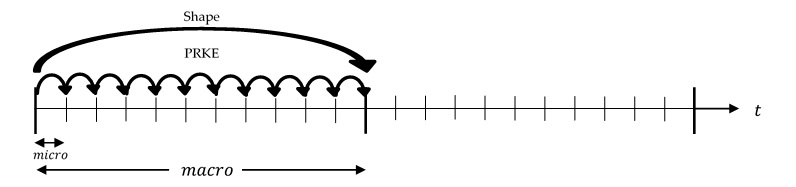
\includegraphics[width=\linewidth]{IQS_visualization.jpg}
\caption{IQS method visualization}
\label{fig:iqsviz}
\end{figure}

It is important to note that the PRKE parameters are evaluated at each macro step and linearly interpolated for the PRKE evaluation. In order to preserve the error convergence of high order discretization schemes for shape, higher order interpolation of the parameters is required.

%%%%%%%%%%%%%%%%%%%%%%%%%%%%%%%%%%%%%%%%%%%%%%%%%%%%%%%%%%%%%%%%%%%%%%%%%%%%%%%%
\subsection{IQS Predictor-Corrector (IQS P-C)}

To avoid performing the IQS non-linear solve, a predictor-corrector version of IQS has been derived in \cite{Dulla2008}. One first solves the neutron flux (represented by Equations \ref{eq:flux} and \ref{eq:precursor}) to obtain a predicted flux. The predicted flux is then converted to a shape through a rescaling argument :
\be
\varphi^g_{n+1} = \underbrace{\phi^g_{n+1}}_{\text{predicted}} \frac{K_0}{K_{n+1}}
\label{eq:rescale}
\ee
Where:
\be
K_{n+1} =\sum_{g=1}^G\left(\phi^{*g},\frac{1}{v^g}\phi^g_{n+1}\right)
\ee
\be
K_{0} =\sum_{g=1}^G\left(\phi^{*g},\frac{1}{v^g}\varphi^g_{n+1}\right)=\sum_{g=1}^G\left(\phi^{*g},\frac{1}{v^g}\phi^g_{0}\right)
\ee

The PRKE parameters are then computed with this shape using Equations \eqref{eq:rmb}-\eqref{eq:l} and interpolated over the macro step for the solution of the PRKE equations.  With the newly computed amplitude, the shape is rescaled and the corrected flux is evaluated:
\be
\underbrace{\phi^g_{n+1}}_{\text{corrected}} = p_{n+1} \times \varphi^g_{n+1} \,.
\ee

%%%%%%%%%%%%%%%%%%%%%%%%%%%%%%%%%%%%%%%%%%%%%%%%%%%%%%%%%%%%%%%%%%%%%%%%%%%%%%%%
\subsection{IQS Solution Process with Multiphysics}

Other physical quantities, such as temperature, are affected by reaction rates and subsequently affect the operators of the flux equations.  
For IQS, this feedback affects both the shape equation and the parameters of the PRKE; thus, it is an additional nonlinear component to the 
already non-linear shape-amplitude equations.  Each of these components have different temporal dependencies; so it may be beneficial for 
efficiency to evaluate them on different time scales.  The amplitude is more rapidly varying than the shape which is computationally expensive to evaluate
and is evaluated only on macro-time steps. In multiphysics simulations, one may take advantage of a fine-scale power distribution in the coupled
physics components (temperature). Figure~\ref{fig:time} shows a such a solution process for temperature feedback.

\begin{figure}[htbp!]
\centering
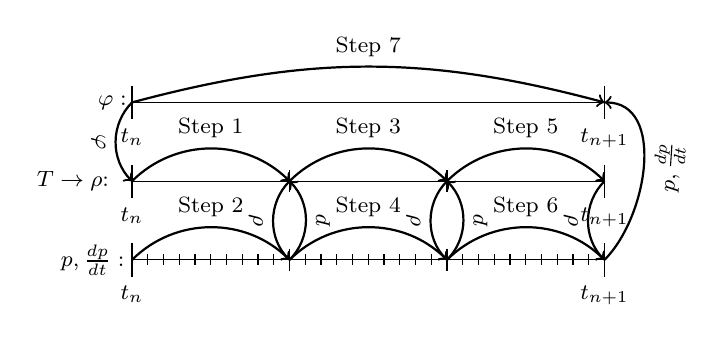
\begin{tikzpicture}[scale=1]
\tikzset{font={\footnotesize}}
%Shape
\draw[] (0,2) -- (6,2) ;
\foreach \x in  {0,6}
\draw[shift={(\x,2)},color=black] (0pt,6pt) -- (0pt,-6pt);
\draw[shift={(0,2)},color=black] (0pt,0pt) -- (0pt,-6pt) node[below] {$t_n$};
\draw[shift={(6,2)},color=black] (0pt,0pt) -- (0pt,-6pt) node[below] {$t_{n+1}$};
\node(shape) at (-.25,2) {$\varphi:$};

%Temp/Params
\draw[] (0,1) -- (6,1) ;
\foreach \x in  {0,6}
\draw[shift={(\x,1)},color=black] (0pt,6pt) -- (0pt,-6pt);
\foreach \x in  {2,4}
\draw[shift={(\x,1)},color=black] (0pt,4pt) -- (0pt,-4pt);
\draw[shift={(0,1)},color=black] (0pt,0pt) -- (0pt,-6pt) node[below] {$t_n$};
\draw[shift={(6,1)},color=black] (0pt,0pt) -- (0pt,-6pt) node[below] {$t_{n+1}$};
\node(temp) at (-.75,1) {$T \rightarrow \rho$:};

% PRKE
\draw[] (0,0) -- (6,0) ;
\foreach \x in  {0,6}
\draw[shift={(\x,0)},color=black] (0pt,6pt) -- (0pt,-6pt);
\foreach \x in  {0,2,4,6}
\draw[shift={(\x,0)},color=black] (0pt,4pt) -- (0pt,-4pt);
\foreach \x in  {0,0.2,0.4,0.6,0.8,1,1.2,1.4,1.6,1.8,2,2.2,2.4,2.6,2.8,3,3.2,3.4,3.6,3.8,4,4.2,4.4,4.6,4.8,5,5.2,5.4,5.6,5.8,6}
\draw[shift={(\x,0)},color=black] (0pt,2pt) -- (0pt,-2pt);
\draw[shift={(0,0)},color=black] (0pt,0pt) -- (0pt,-6pt) node[below] {$t_n$};
\draw[shift={(6,0)},color=black] (0pt,0pt) -- (0pt,-6pt) node[below] {$t_{n+1}$};
\node(prke) at (-.5,0) {$p, \frac{dp}{dt}:$};

\draw (0,0) edge[out=45,in=135,->,thick] node[above,sloped] {Step 2} (2,0);
\draw (2,0) edge[out=45,in=135,->,thick] node[above,sloped] {Step 4} (4,0);
\draw (4,0) edge[out=45,in=135,->,thick] node[above,sloped] {Step 6} (6,0);
\draw (0,1) edge[out=45,in=135,->,thick] node[above,sloped] {Step 1} (2,1);
\draw (2,1) edge[out=45,in=135,->,thick] node[above,sloped] {Step 3} (4,1);
\draw (4,1) edge[out=45,in=135,->,thick] node[above,sloped] {Step 5} (6,1);
\draw (0,2) edge[out=15,in=165,->,thick] node[above,sloped] {Step 7} (6,2);

\draw (0,2) edge[out=-135,in=135,->,thick] node[below,sloped] {$\varphi$} (0,1);
\draw (2,1) edge[out=-135,in=135,->,thick] node[below,sloped] {$\rho$} (2,0);
\draw (2,0) edge[out=45,in=-45,->,thick] node[below,sloped] {$p$} (2,1);
\draw (4,1) edge[out=-135,in=135,->,thick] node[below,sloped] {$\rho$} (4,0);
\draw (4,0) edge[out=45,in=-45,->,thick] node[below,sloped] {$p$} (4,1);
\draw (6,1) edge[out=-135,in=135,->,thick] node[below,sloped] {$\rho$} (6,0);
\draw (6,0) edge[out=45,in=0,->,thick] node[below,sloped] {$p, \frac{dp}{dt}$} (6,2);

\end{tikzpicture}
\caption{Time scales and process of IQS}
\label{fig:time}
\end{figure}

The top time scale represents a shape diffusion evaluation on a macro step, the middle has an arbitrary three steps within the macro step where temperature and the PRKE parameters are evaluated, and the bottom one represents the PRKE evaluation on micro steps.  The shape is linearly interpolated within the macro step for the temperature and PRKE parameter evaluation, and the parameters are interpolated within the temperature step for the PRKE evaluation.  Since there is a nonlinear coupling between all these components, each temperature step is iterated until amplitude has converged and the macro step is iterated until shape has converged. \fig{fig:proc} further visualizes this process as a programming structure.

\begin{figure}[!htpb]
\centering
\resizebox{\linewidth}{!}{%
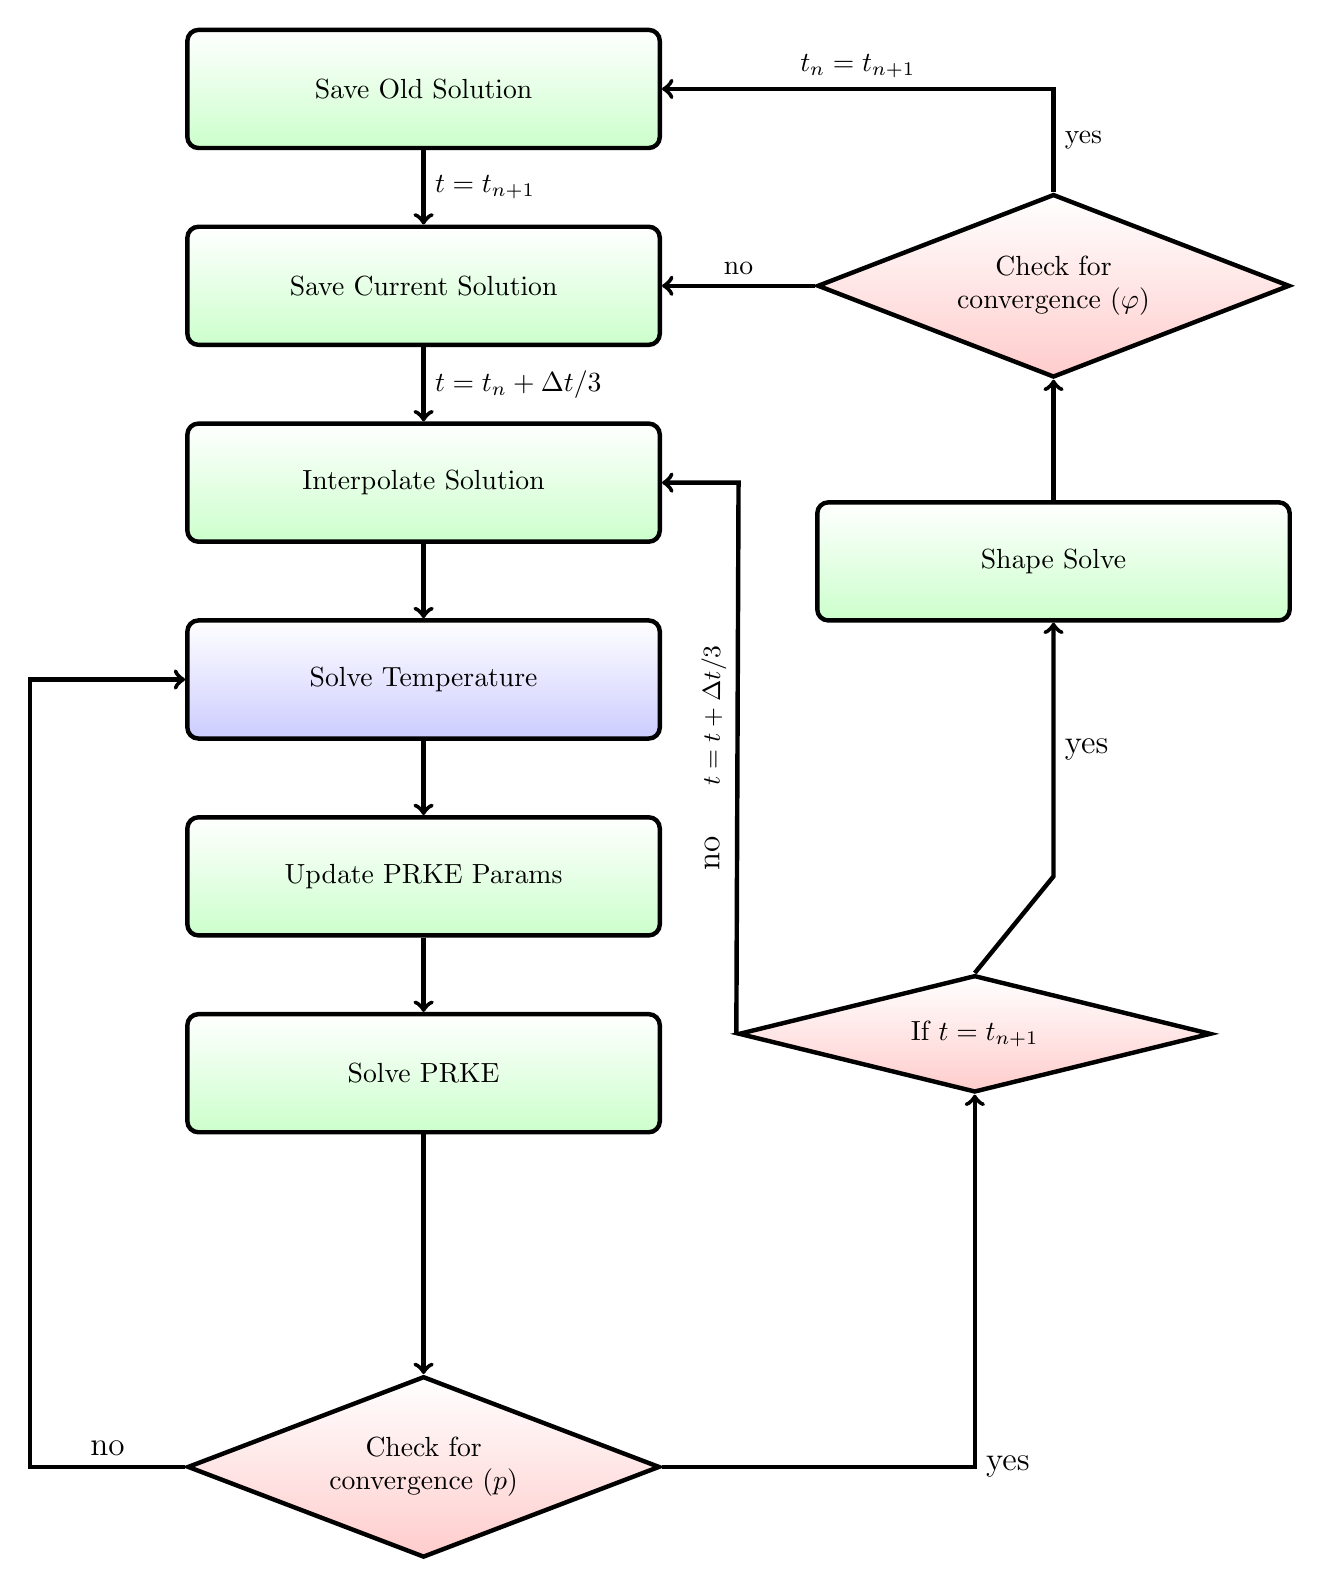
\begin{tikzpicture}[every node/.style = {font=\normalsize}]

\node[greenblock](p1) at (0,0) {Save Old Solution};
\node[greenblock](p2) at (0,-2.5) {Save Current Solution};
\node[greenblock](p3) at (0,-5) {Interpolate Solution};
\node[blueblock](p4) at (0,-7.5) {Solve Temperature};
\node[greenblock] (p5) at (0,-10) {Update PRKE Params};
\node[greenblock] (p6) at (0,-12.5) {Solve PRKE};
\node[reddiamond] (check1) at (0,-17.5) {Check for \\ convergence ($p$)};
\node[reddiamond] (check2) at (7,-12) {If $t=t_{n+1}$};
\node[greenblock] (p7) at (8,-6) {Shape Solve};
\node[reddiamond] (check3) at (8,-2.5) {Check for \\ convergence ($\varphi$)};
%\node [above =0.1mm of p1] {\large{IQS Solve:}};
%\node [above =0.1mm of p5] {\large{Multi-physics:}};

%\tikzback{p1}{p1}{p4}{p4}{bk1}
%\tikzback{p5}{p5}{p5}{p5}{bk2}

\draw[->,ultra thick](p1.south) -- node[right] {$t=t_{n+1}$}(p2.north);
\draw[->,ultra thick](p2.south) -- node[right] {$t=t_{n}+\Delta t/3$}(p3.north);
\draw[->,ultra thick](p3.south) -- (p4.north);
\draw [->,ultra thick] (p4.south)-- (p5.north);
\draw[->,ultra thick](p5.south) -- (p6.north);
\draw[->,ultra thick](p6.south) -- (check1.north);
\draw[->,ultra thick](check1.west) -- node[above,sloped] {\large{no}} (-5,-17.5) |-  (p4.west);
\draw[->,ultra thick](check1.east) -| node[right] {\large{yes}} (check2.south);
\draw[->,ultra thick](check2.west) -- node[above,sloped] {\large{no}\small \qq $t=t+\Delta t/3$} (4,-5) -- (p3.east);
\draw[->,ultra thick](check2.north) --  (8,-10) -- node[right] {\large{yes}} (p7.south);
\draw[->,ultra thick](p7.north) -- (check3.south);
\draw[->,ultra thick](check3.west) -- node[above] {no} (p2.east);
\draw[->,ultra thick](check3.north) -- node[right] {yes} (8,0) -- node[above] {$t_n=t_{n+1}$} (p1.east);

\end{tikzpicture}}
\caption{Visualization of shape iteration and temperature update process for IQS}
\label{fig:proc}
\end{figure}


%%%%%%%%%%%%%%%%%%%%%%%%%%%%%%%%%%%%%%%%%%%%%%%%%%%%%%%%%%%%%%%%%%%%%%%%%%%%%%%%
\section{Results and Analysis}
%%%%%%%%%%%%%%%%%%%%%%%%%%%%%%%%%%%%%%%%%%%%%%%%%%%%%%%%%%%%%%%%%%%%%%%%%%%%%%%%

To test the multiple time scale implementation of IQS, the LRA benchmark was chosen for reference and a TREAT example was employed. 

%%%%%%%%%%%%%%%%%%%%%%%%%%%%%%%%%%%%%%%%%%%%%%%%%%%%%%%%%%%%%%%%%%%%%%%%%%%%%%%%
\subsection{LRA Benchmark}

The LRA benchmark is a two-dimensional, two-group neutron diffusion problem with adiabatic heat-up and Doppler feedback in thermal reactor \cite{ANL_BPB}.  It is a super prompt-critical transient. The execution of the benchmark was performed by the Rattlesnake/MOOSE framework at Idaho National Laboratory (INL).  The spacial discretization was performed using continuous finite element method with first order Lagrangian basis functions. The mesh consisted of blocks 11X11 with five uniform refinements, totaling 165,165 elements and 124,609 nodes. Three different temporal techniques were applied: implicit discretization of the flux equation (Brute force), IQS, and IQS-PC. Crank-Nicholson time discretization scheme was used for the diffusion evaluation of each technique.  Third order Runge–Kutta discretization with step doubling adaptation was used for the PRKE evaluation.  The performance of IQS and the temperature updates were measured by its improvement in accuracy at peak power over the Brute force technique.

%%%%%%%%%%%%%%%%%%%%%%%%%%%%%%%%%%%%%%%%%%%%%%%%%%%%%%%%%%%%%%%%%%%%%%%%%%%%%%%%
\subsubsection{LRA Temperature Feedback}
\label{sec:LRA_T}

The heat up is described by \eqt{eq:temp} and the feedback is described by \eqt{eq:dopp}.

\be
\rho c_p \frac{\partial T(\vec{r},t)}{\partial t} = \kappa_f \sum^G_{g=1}\Sigma_f^g \phi^g(\vec{r},t)
\label{eq:temp}
\ee

\be
\Sigma_a^{thermal}(\vec{r},t) = \Sigma_a^{thermal}(\vec{r},0)\left[1+\gamma\left(\sqrt{T}-\sqrt{T_0}\right)\right]
\label{eq:dopp}
\ee

In the temperature evaluation, a typical implicit solver would simply use the interpolated flux at end of the temperature time step for the right hand side of the equation.  However, IQS has much more information about the profile of the flux along the time step because of the micro-step amplitude evaluation.  Therefore, it is possible to solve for temperature using a semi-analytical approach, shown by \eqt{eq:temp_an}.

\be
T^{n+1} = T^n + \frac{\kappa_f}{\rho c_p} \left(a_2 \varphi^{n+1} + a_1 \varphi^{n}\right)
\label{eq:temp_an}
\ee
Where $n$ corresponds to the beginning of the temperature step.  $a_1$ and $a_2$ are integration coefficients defined by \eqt{eq:a1} and \eqt{eq:a2}.
\be
a_1 = \int_{t_n}^{t_{n+1}}\left(\frac{t_{n+1}-t'}{\Delta t}\right)p(t')dt'
\label{eq:a1}
\ee
\be
a_2 = \int_{t_n}^{t_{n+1}}\left(\frac{t'-t_n}{\Delta t}\right)p(t')dt'
\label{eq:a2}
\ee

Any interpolation of the amplitude along the micro steps is possible for the integration, this application uses piece-wise linear.

%%%%%%%%%%%%%%%%%%%%%%%%%%%%%%%%%%%%%%%%%%%%%%%%%%%%%%%%%%%%%%%%%%%%%%%%%%%%%%%%
\subsubsection{LRA Results}

\fig{fig:lra_profile} shows the baseline power and temperature profile for the LRA benchmark.  The baseline results are compared to the results achieved by Sutton and Aviles in \cite{Sutton_1996} and presented in \tbl{tab:base}.  The relative difference in the magnitude of the peak power ($t\approx1.44 s$) from the baseline was used for error comparison.  \fig{fig:lra_bad} is an error convergence plot comparing the three techniques where temperature is evaluated only on the macro step (1 temperature update).  \fig{fig:conv} is an error convergence plot comparing the three techniques where temperature is evaluated 5 times within a macro step (5 temperature updates).  Finally, \fig{fig:mp} shows the affect of various temperature updates. The dashed lines correspond to brute force at different flux step sizes, while the IQS macro step size is kept constant. \\

\begin{figure}[htbp!]
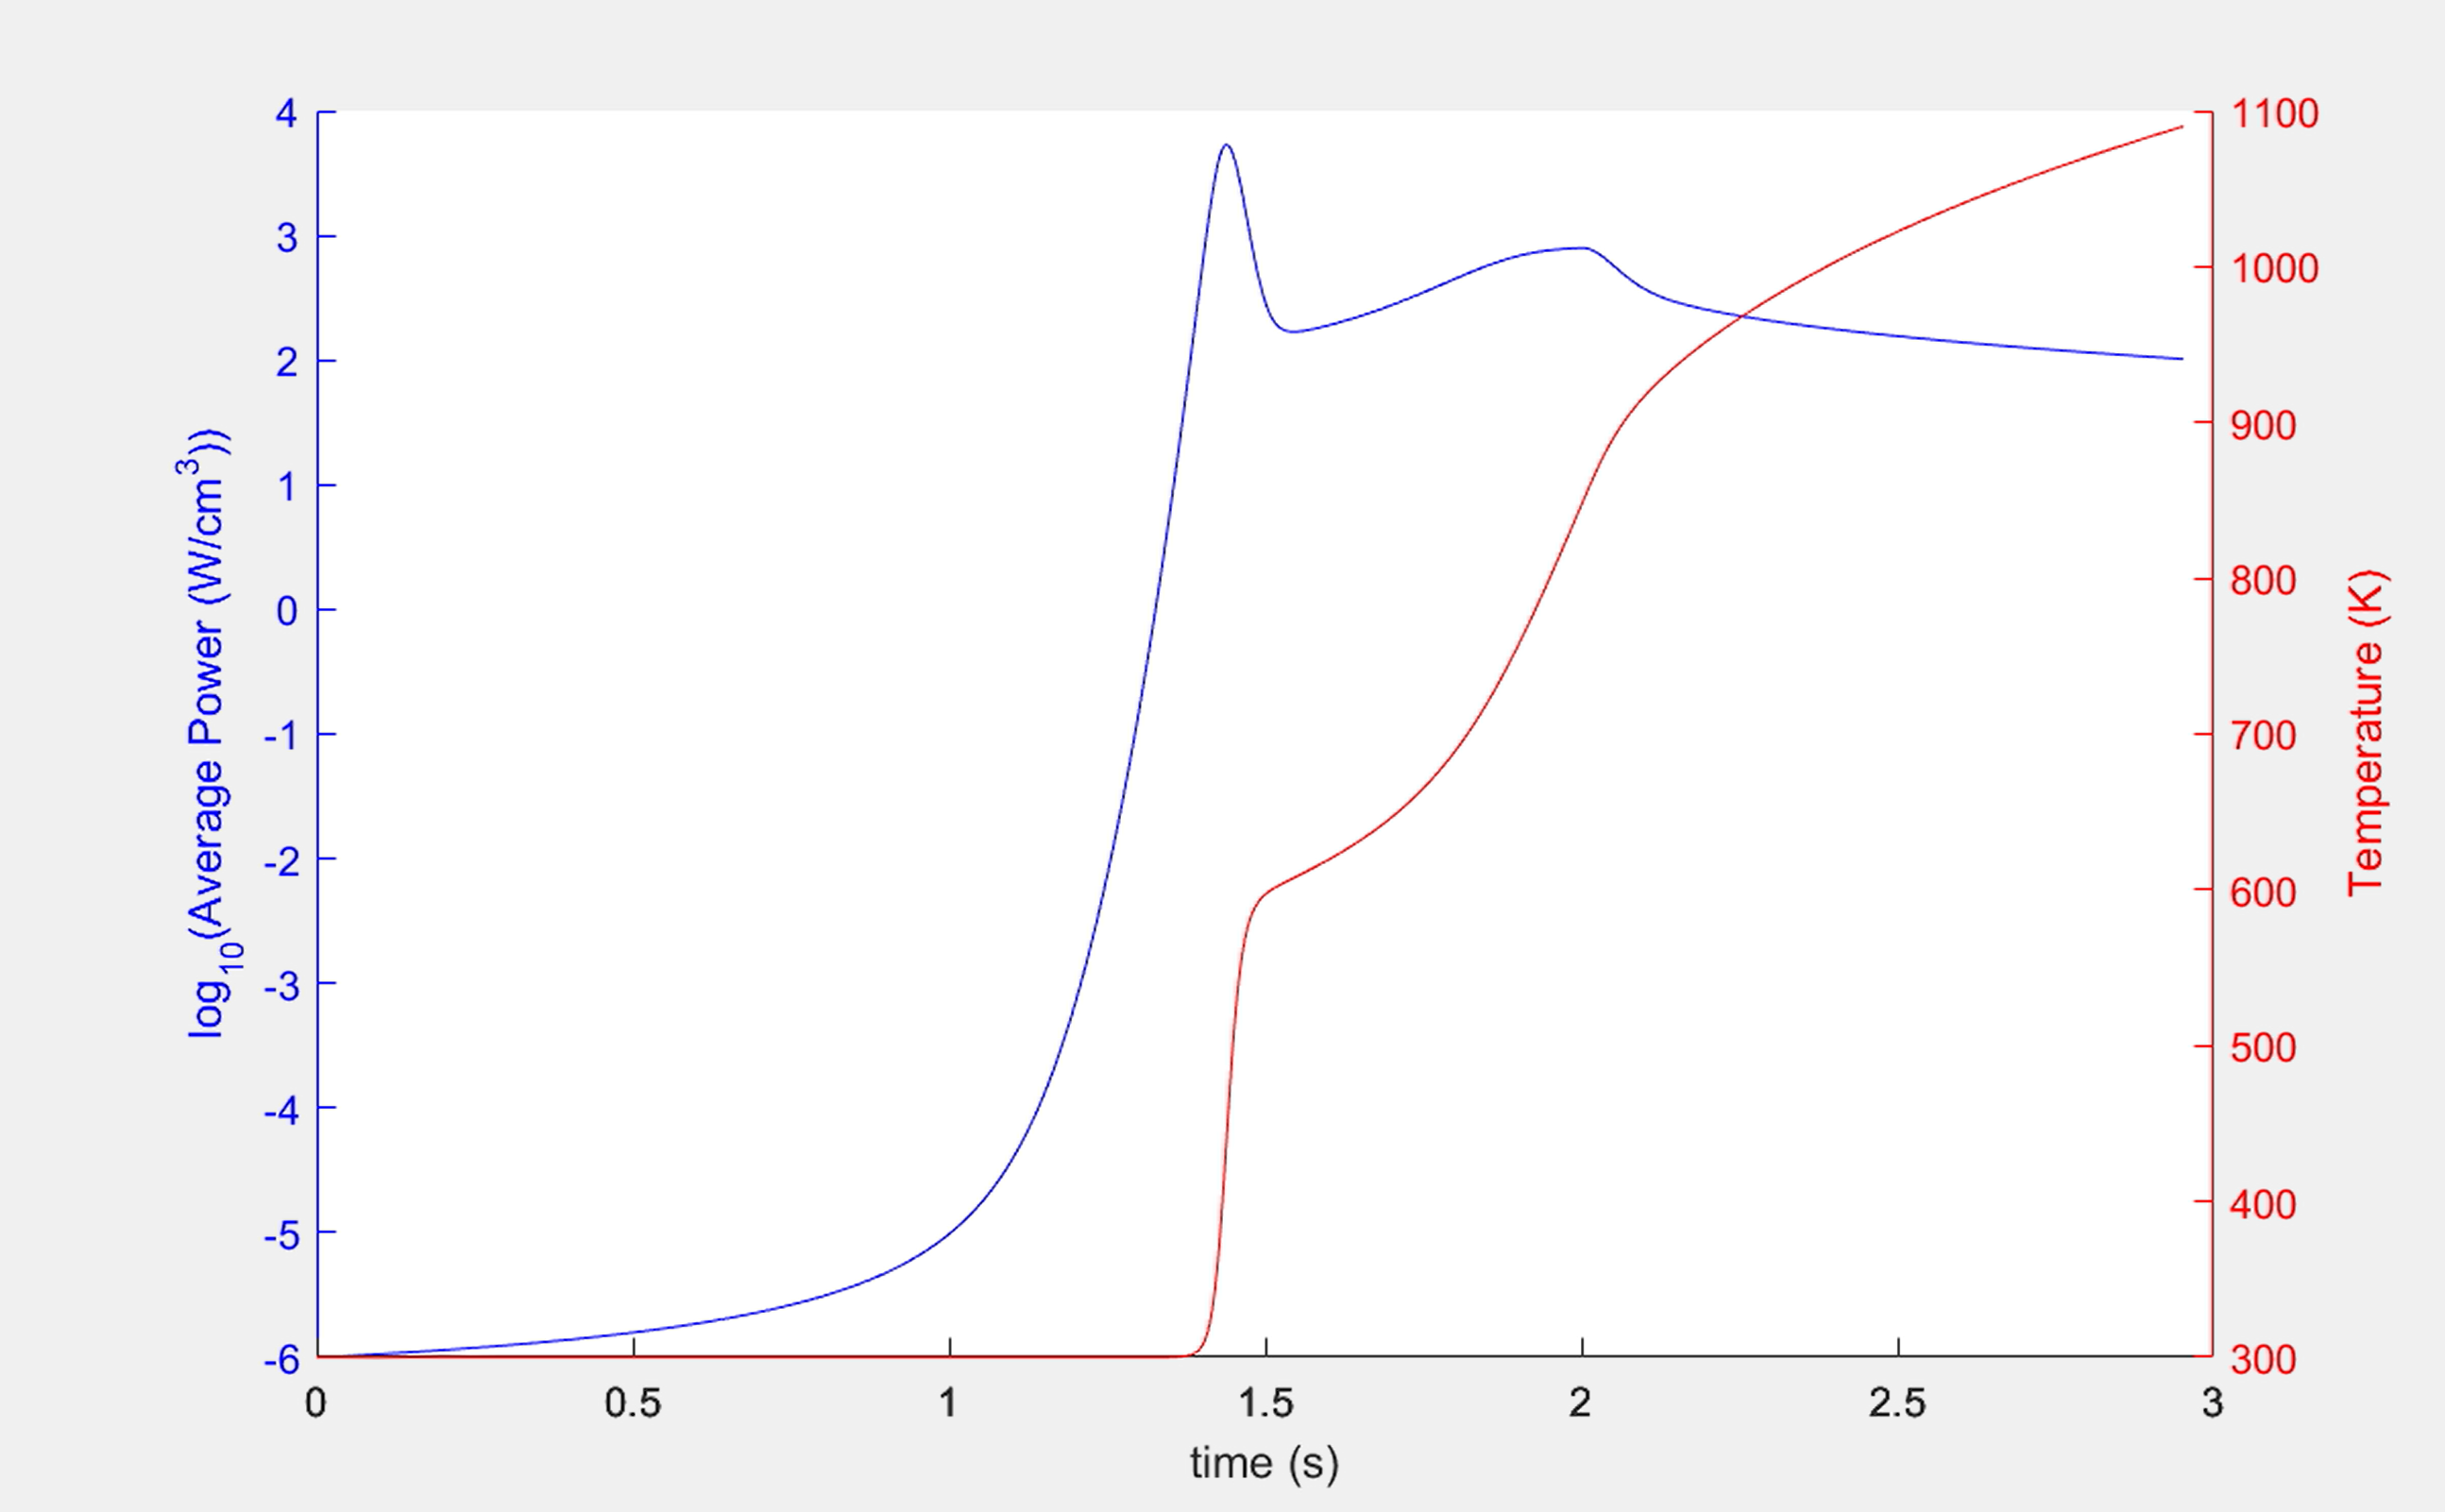
\includegraphics[width=\linewidth]{lra_profile.png}
\caption{LRA baseline temperature and power profile}
\label{fig:lra_profile}
\end{figure}

\begin{table}[!htbp]
\begin{center}
\resizebox{\linewidth}{!}{
\begin{tabular}{|l|cc|}
\hline
Calculation  &  Baseline & Sutton (Spandex 1936) \\
\hline
No. of Mesh 			& 3872 		& 1936 \\
Eigenvalue 				& 0.99637	& 0.99637 \\
No. of Time Steps 		& 6000 		& 23,890 \\
Time to Peak Power (s) 	& 1.441 	& 1.441 \\
Peak Power (W/cm$^3$) 	& 5456 		& 5461 \\
\hline
\end{tabular}
}
\end{center}
\caption{LRA baseline verification}
\label{tab:base}
\end{table}

\begin{figure}[!htpb]
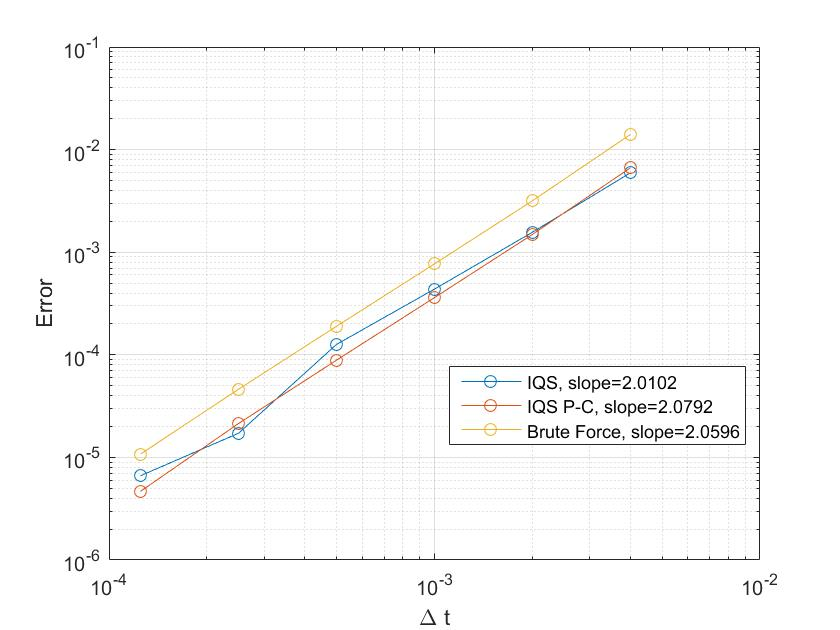
\includegraphics[width=\linewidth]{lra_bad.jpg}
\caption{LRA convergence plots with only one temperature update each macro step}
\label{fig:lra_bad}
\end{figure}

\begin{figure}[htbp!]
\centering
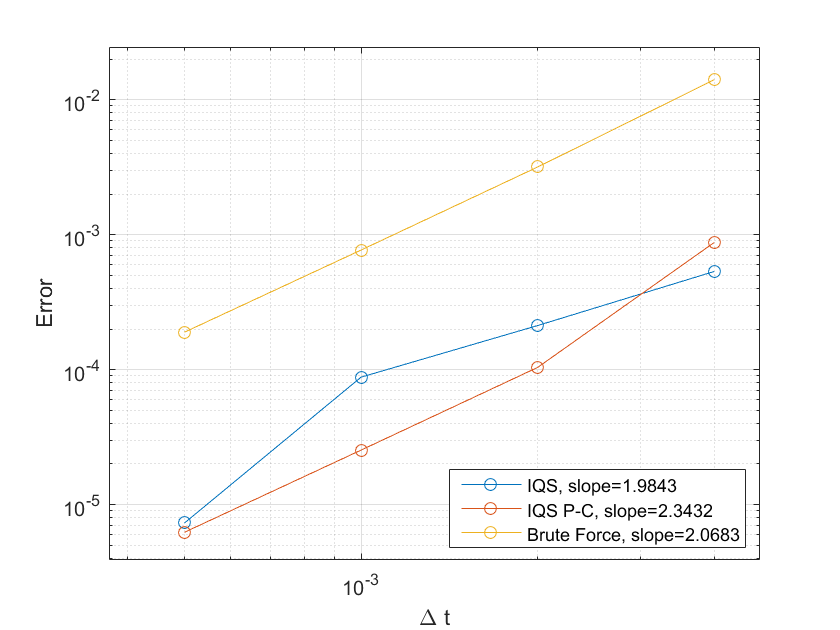
\includegraphics[width=\linewidth]{lra_mp_convergence.png}
\caption{Error convergence plot with 5 temperature updates per macro step}
\label{fig:conv}
\end{figure}

\begin{figure}[htbp!]
\centering
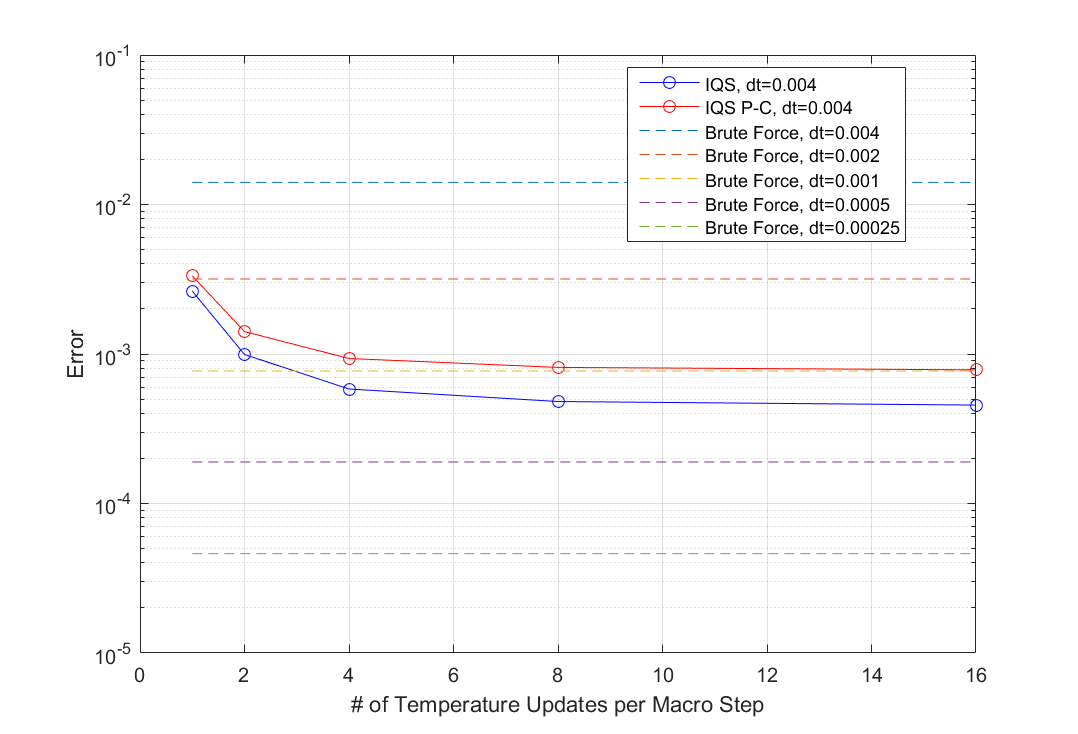
\includegraphics[width=\linewidth]{lra_mp.png}
\caption{Error plot with various temperature updates per macro step}
\label{fig:mp}
\end{figure}

The convergence plots show that updating temperature and the PRKE parameters within a macro step has a significant affect on the performance of IQS.  With only one update, IQS was only slightly better than brute force, brute force required about 150\% more time steps than IQS for the same error.  While 5 temperature updates showed a much more significant IQS performance, brute force required about 400\% more time steps than IQS for the same error.  \fig{fig:mp} shows that error has a convergent behavior for the number of temperature updates.  This convergence makes sense because temperature can only be so accurate before the error in shape is dominating. Table \ref{tab:ndiff_lra} shows the run time results for the implicit discretization calculations.  Tables \ref{tab:iqs_lra} and \ref{tab:iqspc_lra} present the IQS run-times with various numbers of temperature updates.  These run-times are based on total alive time of the execution where the diffusion evaluation is distributed over 24 processors. \\

\begin{table}[!htbp]
\begin{center}
%\resizebox{\linewidth}{!}{
\begin{tabular}{|l|l|cc|}
\hline
Run  &  $\Delta t$ & Error & Runtime (hr) \\
\hline
1	& 4.0e-3	& 1.407e-2 	& 4.11	\\
2	& 2.0e-3	& 3.174e-3 	& 5.68 	\\
3 	& 1.0e-3 	& 7.690e-4 	& 5.55	\\
4 	& 5.0e-4 	& 1.892e-4 	& 13.57	\\
5 	& 2.5e-4	& 4.590e-5 	& 23.81	\\
\hline
\end{tabular}
%}
\end{center}
\caption{Implicit discretization run time results}
\label{tab:ndiff_lra}
\end{table}

\begin{table}[!htbp]
\begin{center}
%\resizebox{\linewidth}{!}{
\begin{tabular}{|l|l|ccc|}
\hline
	&  Temperature 	&  		& Runtime 	& \% Increase	\\
Run	&  Updates 	& Error & (hr)		& in Runtime$^*$\\
\hline
1	& 1		& 2.612e-3 	&  `&	\\
2	& 2		& 9.893e-4 	& 	& 	\\
3 	& 4 	& 5.796e-4 	& 	&	\\
4 	& 8 	& 4.772e-4 	& 	&	\\
5 	& 16	& 4.516e-4 	& 	&	\\
\hline
\end{tabular}
%}
\end{center}
\caption{Traditional IQS run time results with $\Delta t = 0.004$}
\label{tab:iqs_lra}
\end{table}

\begin{table}[!htbp]
\begin{center}
%\resizebox{\linewidth}{!}{
\begin{tabular}{|l|l|ccc|}
\hline
	&  Temperature 	&  		& Runtime 	& \% Increase	\\
Run	&  Updates 	& Error & (hr)		& in Runtime$^*$\\
\hline
1	& 1		& 3.488e-3 	& 6.24 `&	\\
2	& 2		& 1.349e-3 	& 6.18	& 	\\
3 	& 4 	& 9.161e-4 	& 7.05	&	\\
4 	& 8 	& 8.052e-4 	& 7.72	&	\\
5 	& 16	& 7.905e-4 	& 10.82	&	\\
\hline
\end{tabular}
%}
\end{center}
\caption{IQS PC run time results with $\Delta t = 0.004$}
\label{tab:iqspc_lra}
\end{table}

%%%%%%%%%%%%%%%%%%%%%%%%%%%%%%%%%%%%%%%%%%%%%%%%%%%%%%%%%%%%%%%%%%%%%%%%%%%%%%%%
\subsection{Transient-15 TREAT Example}

Transient 15 is a small core TREAT experiment that was modeled by the Rattlesnake group at INL for demonstrating their model's fidelity to TREAT’s feedback mechanisms. The goal of the simulations is to obtain a power peak whose position and magnitude that sufficiently matches experimental results.  The model involves an 11 energy group diffusion approximation and is discretized into 355,712 hexahedral continuous finite elements totaling 4,109,523 degrees of freedom.  The three second transient involves a linear ramp decrease in boron content throughout the fuel region.  \fig{fig:Tran15} shows a visualization of the flux profile within the core, hidden is the massive amount of graphite surrounding the core.   

\begin{figure}[htbp!]
\centering
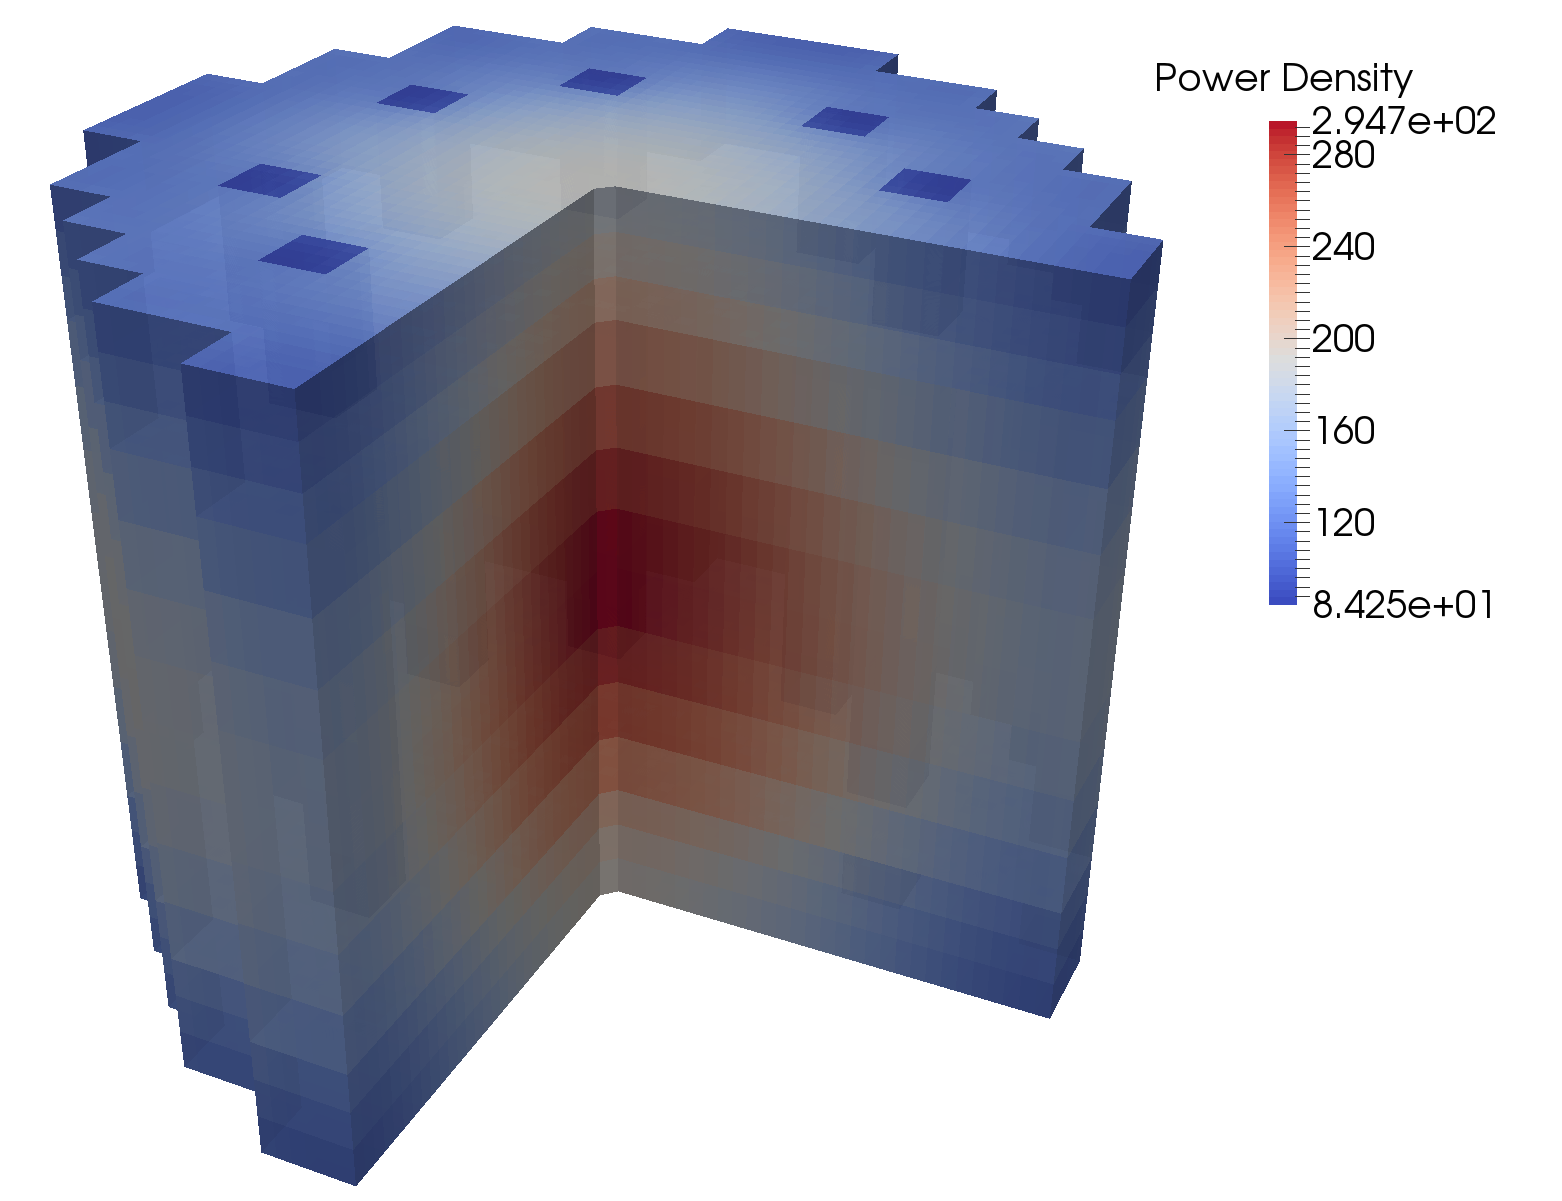
\includegraphics[width=\linewidth]{Tran15_core2.png}
\caption{Transient 15 core power profile at peak power}
\label{fig:Tran15}
\end{figure}


%%%%%%%%%%%%%%%%%%%%%%%%%%%%%%%%%%%%%%%%%%%%%%%%%%%%%%%%%%%%%%%%%%%%%%%%%%%%%%%%
\subsubsection{Transient-15 Temperature Feedback}

The Transient-15 model uses a adiabatic temperature feedback mechanism, similar to the one explored by the LRA. \eqt{eq:temp2} describes the heat up of the fuel.  It is very similar, except the specific heat is now dependent on temperature is described by \eqt{eq:cp}.  The temperature evaluation is identical to the one described in LRA section, except a Newton iteration process is employed to resolve the nonlinearity from the specific heat term.  The feedback to the cross-sections are applied using linear interpolation of tabular data provided by INL.

\be
\rho c_p(T) \frac{\partial T(\vec{r},t)}{\partial t} = \kappa_f \sum^G_{g=1}\Sigma_f^g \phi^g(\vec{r},t)
\label{eq:temp2}
\ee

\be
c_p = -5.8219e-10T^3 - 4.3694e-7T^2 + 2.8369e-3T -1.009e-2
\label{eq:cp}
\ee

%%%%%%%%%%%%%%%%%%%%%%%%%%%%%%%%%%%%%%%%%%%%%%%%%%%%%%%%%%%%%%%%%%%%%%%%%%%%%%%%
\subsubsection{Transient-15 Results}

\fig{fig:Tran15_profile} shows the baseline power and temperature profile for the Transient-15 example.

\begin{figure}[htbp!]
\centering
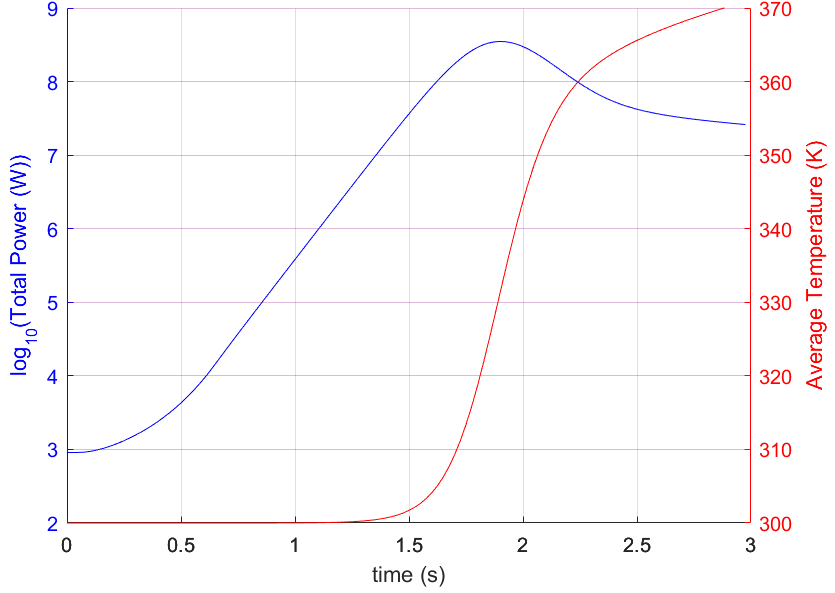
\includegraphics[width=\linewidth]{Tran15_profile.png}
\caption{Transient 15 total power and average temperature profile during transient}
\label{fig:Tran15_profile}
\end{figure}

%%%%%%%%%%%%%%%%%%%%%%%%%%%%%%%%%%%%%%%%%%%%%%%%%%%%%%%%%%%%%%%%%%%%%%%%%%%%%%%%
\section{Conclusions}

IQS is a powerful tool for reactor simulation, it has the capability of greatly reducing computation time while retaining accuracy of relevant quantities.  The goal of this summary is to demonstrate IQS's performance with multi-physics simulations, as well as techniques to improve its performance.  The technique focused on incorporating a new time scale in IQS for feedback quantities and PRKE parameters.  The results when IQS is applied to the temperature feedback model of the LRA benchmark showed that incorporating a intermediate time scale for temperature has significant impact on IQS performance.

The full paper version will include time adaptive simulations for multiphysics dynamic transients: LRA benchmark, a full core TREAT model, and the Lady Godiva benchmark with structural feedback \cite{CritSafetyHandbook}. Performance of the IQS method with intermediate time scale for physics feedback will be compared to that of an implicit discretization of the flux equations with feedback. 

%%%%%%%%%%%%%%%%%%%%%%%%%%%%%%%%%%%%%%%%%%%%%%%%%%%%%%%%%%%%%%%%%%%%%%%%%%%%%%%%
%\appendix
%\section{Appendix}

%%%%%%%%%%%%%%%%%%%%%%%%%%%%%%%%%%%%%%%%%%%%%%%%%%%%%%%%%%%%%%%%%%%%%%%%%%%%%%%%
\section{Acknowledgments}
This work was supported by the Department of Energy, Idaho National Laboratory, and the Integrated University Program Fellowship.  We thank Mark Dehart, Yaqi Wang, the NEAMS program, and INL's Moose/Rattlesnake team for their support.

%%%%%%%%%%%%%%%%%%%%%%%%%%%%%%%%%%%%%%%%%%%%%%%%%%%%%%%%%%%%%%%%%%%%%%%%%%%%%%%%
\bibliographystyle{ans}
\bibliography{references_IQS}

\end{document}

